\chapter{Literature Review}

\vspace{-15mm}
\section{Servomotors}
\vspace{-5mm}
Typically servomotors are rotary or linear actuators that are controlled using a microcontroller and an encoder. This allows for the precise angular position, velocity and/or acceleration control of the output shaft. Servomotors are commonly used in motoring applications such as 3D printing and CNC machines, or in robotic arms and assemblies which use forward and reverse kinematics in order control specific motor positions allowing for complex tasks to be completed accurately\cite{servo}.
\vspace{-5mm}
\begin{figure}[H]
  \centering
  \begin{minipage}[b]{0.45\textwidth}
  \centering
    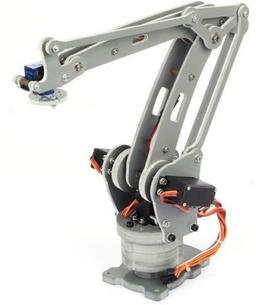
\includegraphics[width=0.35\textwidth]{servo_arm.jpg}
    \caption{Servo controlled arm  \cite{servo_arm}}
  \end{minipage}
  \hfill
  \begin{minipage}[b]{0.45\textwidth}
    \centering
    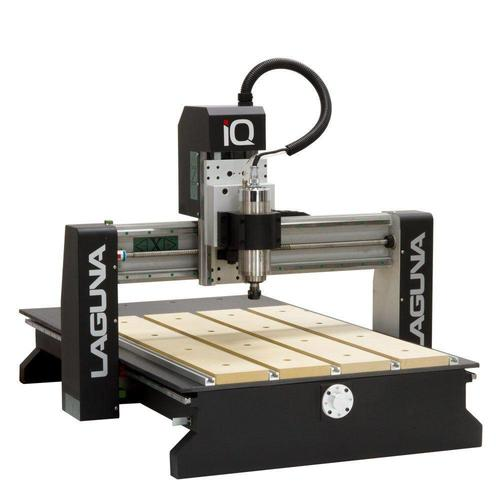
\includegraphics[width=0.5\textwidth]{cnc.jpg}
    \caption{CNC machine \cite{cnc}}
  \end{minipage}
\end{figure}
\vspace{-8mm}
A servomotors usually has 3 wires, Control, Power and Ground. The output shafts angle is controlled through adjusting the duty cycle of a Pulse Width Modulated (PWM) signal being supplied to its control wire. The on board microchip receives this signal and in turn outputs a voltage to a DC motor based on the duty cycle of the signal. This voltage rotates the motors shaft, which in turn rotates the output shaft to a specific angle, usually  between 0\degree and 180\degree but there are also servos that have it outputs a voltage 360\degree  of rotation. This position is tracked and controlled using an encoder such as a potentiometer in order to determine current position, but there are many other types of encoders which can give more accurate position, direction of rotation and velocity control. A typical servomotor and its components can be see in Figure \ref{fig:servoexplode} and Table \ref{tab:servomotorcomponents}. 
\vspace{-3mm}
\begin{figure}[H]
  \begin{minipage}[b]{0.48\textwidth}
    \begin{figure}[H]
        \centering
        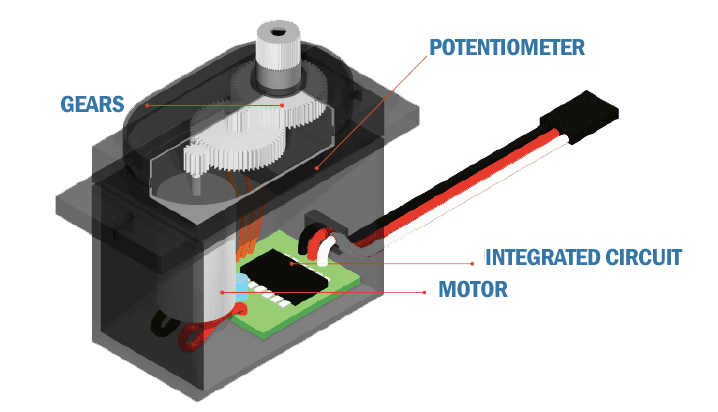
\includegraphics[width=0.8\textwidth]{Servoexploded.png}
        \caption{Servomotor components\cite{servoexplode}}
        \label{fig:servoexplode}
    \end{figure} 
\end{minipage}
\hfill
\begin{minipage}[b]{0.48\textwidth}
  \
    \begin{table}[H]
        \centering
        \begin{tabular}{|l|}
        \hline
        \textbf{\underline{A servomotors components}}\\
             - A Motor(AC/DC) \\
             - Potentiometer as the encoder \\
             - A microcontroller for control \\
             - A Gear train \\
         \hline
        \end{tabular}
    \caption{Servomotor components }
    \label{tab:servomotorcomponents}
    \end{table}
  \end{minipage}
\end{figure}
\vspace{-10mm}

\newpage
\section{DC motors}
A current carrying conductor within a magnetic field will experience a force. The direction of the force will be perpendicular to the plane containing the current carrying conductor and it's magnetic field which are also perpendicular to each other. This is the principle used in a simple brushed DC motor with permanent magnets used for poles and a slip ring commutator to alternate the flow of the current on the conductor. Power to the coils is supplied through fixed conductive brushes that make contact with the rotating commutator. The force rotates the shaft at a rate related to the voltage applied to the motor\cite{DC_Motor}.
\begin{figure}[H]
\centering
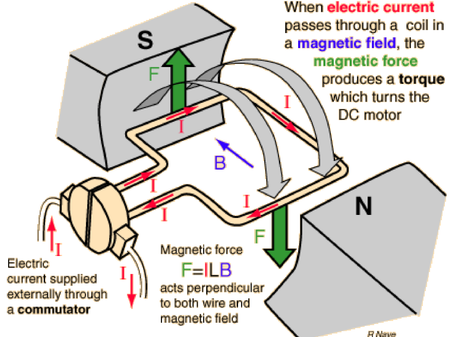
\includegraphics[width=0.5\textwidth]{lorenzforce.png}
\caption{Current carrying conductor in a magnetic field\cite{DCmotor}}
\end{figure} 
With brushless DC motors the rotor is a permanent magnet, the rotor is then rotated by rotating the surrounding magnetic field. Brushless motors have a higher power to weight ratio and high speed control. They do not miss steps and are much more powerful and efficient, but cost a lot more than brushed DC motors  \cite{brushlessDC}
\begin{figure}[H]
\centering
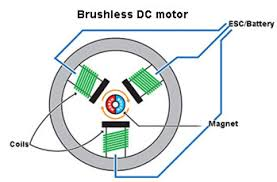
\includegraphics[width=0.45\textwidth]{Brushless_DC.jpeg}
\caption{Brushless DC motor \cite{brushlessDC}}
\end{figure} 


\newpage
\section{Microcontrollers}
A microcontroller acts as the brain of the system, using different peripherals to interact with different devices and being able to make decisions in order to perform tasks. The hardware integrated with microcontroller and the quality of the software loaded determines how well it functions and tasks it can perform.

\subsection{Flash Memory}
Flash memory is an electronic non-volatile computer storage medium that can be electronically erased and reprogrammed. Flash memory contains its information even when the device is not powered. What is included in this is information required to start up the micro and be active during runtime.

The Flash memory on the STM32F051C6 has been organised into 32-bit wide memory cells that can be used for storing both code and data constants.

\textbf{This information is divided into two parts :}
\begin{enumerate}
\item{\textbf{System memory}}
which is used to boot the device on start-up in System memory boot mode. This area is reserved for use by the manufacturers of the microcontroller, and contains the boot loader which is used to reprogram the Flash memory through the selected communication interface. It is programmed by ST when the device is manufactured, and protected against various write/erase operations. 

\item{\textbf{Optional bytes}}
that include those used when re-programming the device for specific applications.
\end{enumerate}

\subsection{DAC}
Digital-to-analog converters are used to create an analog signal based on a digital value. The most basic type of electronic DAC uses pulse-width modulation and a low pass filter. A chosen stable current or voltage is achieved by adjusting the frequency of the PWM signal. The duty cycle of the PWM based on the value of digital input. This technique is often used for electric motor speed controllers and other applications \cite{DAC}.

\newpage
\subsection{ADC}
An analogue-to-digital converter(ADC) allows for a voltage source to be sampled and read in to the microcontroller as digital code. The resolution of the ADC determines the number of bits used to specify a certain voltage range e.g. for an ADC with $2^8$ bit having a resolution 255. If the voltage range to be sample is between 0V and 3.3V. Gives a resolution of 12.9mV per bit.

\subsubsection{Successive Approximation Converters}
Successive approximation ADCs are a type of analog-to-digital converter that reads in a continuous analog signal and outputs a digital binary value based on the input signal. This type of converter uses a binary search through all the possible quantization levels. The SAR outputs a binary value of the approximated ADC value, which is then converted back into an analog signal and compared to the input wave form using a comparator. If the signals are not the same the SAR increments its approximation until converging upon the final digital value to be output. Once this occurs an End Of Conversion (EOC) signal is sent to the microcontroller.

The STM32F051C6 uses a Successive Approximation ADC like the one seen below in Figure \ref{fig:SAC}.
\begin{figure}[H]
    \centering
    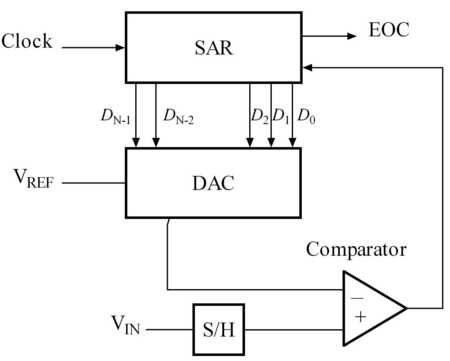
\includegraphics[width=0.5\textwidth]{SA_ADC_block_diagram.jpg}
    \caption{Successive Approximation Converters \cite{SA_converter}}
    \label{fig:SAC}
\end{figure}





\newpage
\section{Sensors}
Multiple sensors will be incorporated into the final design of the controller board. Sensors are important in the functioning and accurate control of the system as well as allowing for protection against overheating and excess current draws. 

\vspace{-7mm}
\subsection{Current sensor}
A current sensor is a device that detects electric current and generates a signal in proportion to that of the current, the output of the sensor can be analogue or digital \cite{current_sensor}. 

\textbf{Typical current sensors that are available:}  
\begin{table}[H]
    \centering
    \begin{tabular}{|c|c|}
    \hline
    &\\
      \begin{minipage}[b]{0.45\textwidth}
            \begin{figure}[H]
                \centering
                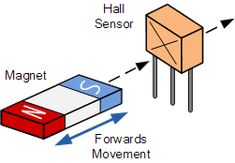
\includegraphics[width=0.5\textwidth]{Hall_Effect.jpg}
                \caption{Hall sensor}
                \label{fig:hall}
            \end{figure}

      \end{minipage}
         & 
      \begin{minipage}[b]{0.45\textwidth}
           \textbf{Hall effect sensors}, seen in Figure 2.7. can be used to measure the magnetic field made created by the current flowing through conductor and from that determine the actual current. \newline
      \end{minipage}\\

      \hline      
      \begin{minipage}[b]{0.45\textwidth}
          \textbf{Shunt resistors}, seen in Figure 2.8. Use Ohms law in order to calculate the current flowing. $V = I\times R$, with a known applied voltage and chosen resistor the current can be calculated.\newline
      \end{minipage}
         &  
        \begin{minipage}[b]{0.45\textwidth}
            \begin{figure}[H]
              \centering               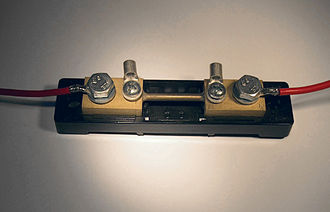
\includegraphics[width=0.6\textwidth]{shunt_resistor.jpg}
                \caption{Shunt resistor}
                \label{fig:shunt}
            \end{figure}
        \end{minipage}\\
        \hline        

          \begin{minipage}[b]{0.45\textwidth}
          \begin{figure}[H]
            \centering
            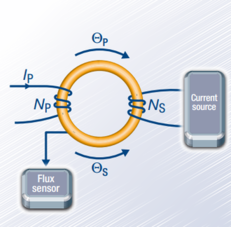
\includegraphics[width=0.5\textwidth]{saturable_inductor.png}
            \caption{Saturable inductor}
            \label{fig:Saturable}
          \end{figure}
          \end{minipage}
         &  
           \begin{minipage}[b]{0.45\textwidth}
            \textbf{Saturable inductor sensors}, seen in Figure 2.9. Work in a similar manner to that of Hall effect sensors in that they measure the change in the magnetic field in order to determine the current flowing through a conductor.
            \vspace{6mm}
          \end{minipage}
         \\
     \hline
    \end{tabular}
    \vspace{2mm}
    \caption{Types of current sensor}
\end{table}


\newpage
\subsection{Encoders}
Encoders are electromechanical devices that output an electrical signal proportional to that of the position of the input shaft.

\textbf{Typical encoders that are available:}  
\vspace{5mm}
\begin{table}[H]
    \vspace{-5mm}
    \centering
    \begin{tabular}{|c|c|}
    \hline
      \begin{minipage}[b]{0.49\textwidth}
      \vspace{2mm}
        \textbf{Optical encoders}, which use pulses of light emitted by infrared diodes shining through slots. This can be seen in Figure 2.10 As the number of slots increases so does the encoders resolution\cite{encoders}.
        \vspace{5mm}
      \end{minipage}
         & 
      \begin{minipage}[b]{0.49\textwidth}
      \begin{figure}[H]
        \centering
        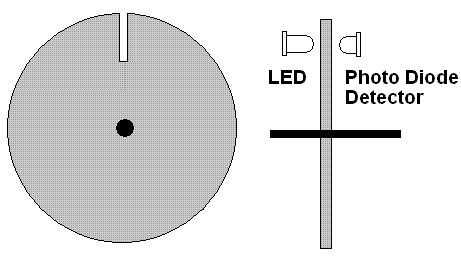
\includegraphics[width=0.6\textwidth]{slottedencoder.png}
        \caption{Optical encoder}
        \label{fig:optical}
      \end{figure}
      \end{minipage}\\
      \hline   
      
      \begin{minipage}[b]{0.45\textwidth}
      \centering
      \begin{figure}[H]
          \centering
            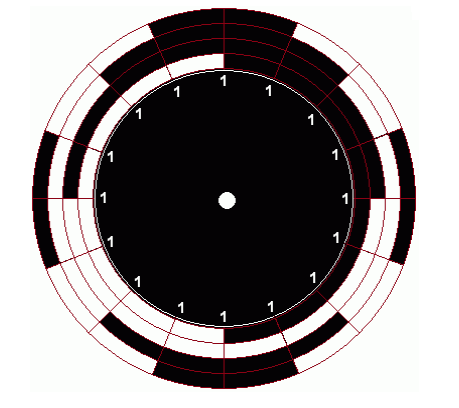
\includegraphics[width=0.49\textwidth]{Graycodeencoder.png}
            \caption{Binary encoder}
            \label{fig:binenc}
      \end{figure}

      \end{minipage}
         &  
        \begin{minipage}[b]{0.49\textwidth}
        \vspace{2mm}
              \textbf{Binary encoders}, which uses a template that has segments based on a binary value to determine current position. This can be seen in Figure 2.11. multiple motor positions can be determined, the number of positions has a $2^N$ relationship with the number of segments in the encoder. 
              \vspace{2mm}
        \end{minipage}\\
         \hline
          \begin{minipage}[b]{0.49\textwidth}         
            \textbf{Potentiometers}, are a mechanical encoder. This can be seen in Figure 2.12. Where the different resistance values and there associated voltage represent different position values of the wiper on the resistive strip \cite{rotarypot}.
        \end{minipage}
         &
          \begin{minipage}[b]{0.49\textwidth}
          \centering
              \begin{figure}[H]
              \centering
                 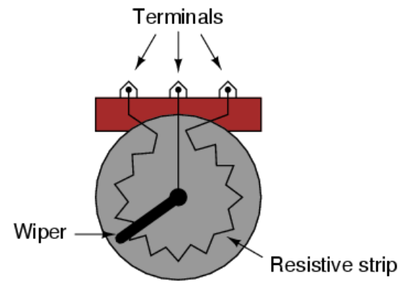
\includegraphics[width=0.5\textwidth]{Rotarypot.png}
                    \caption{Potentiometer}
                    \label{fig:pot}
              \end{figure}

 
        \end{minipage}
         \\
         \hline
          \begin{minipage}[b]{0.49\textwidth}
          \centering
          \begin{figure}[H]
          \centering
             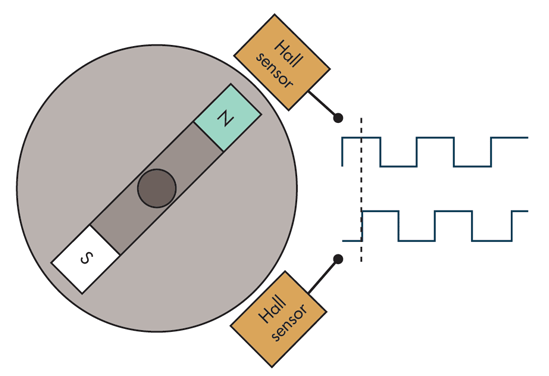
\includegraphics[width=0.4\textwidth]{Halleffect.png}
             \caption{Hall effect encoder}
             \label{fig:hallenc}
          \end{figure}
         \end{minipage}
         &
          \begin{minipage}[b]{0.49\textwidth}
          \vspace{5mm}
          \textbf{Hall effect sensors}, are transducers that have an output voltage that varies in response to a magnetic field. Seen in Figure
          2.13. This us then used to determine position and velocity\cite{halleffect}. 
          \vspace{5mm}
          \end{minipage}
         \\
         
     \hline
    \end{tabular}
    \vspace{-4mm}
    \caption{Types of encoders}
\end{table}
\vspace{-10mm}



\newpage
\subsection{Temperature sensors}
Temperature sensors are an important way to monitor and keep track of the state of the device during different operating conditions.

\begin{itemize}
	\item[-]Analogue temperature sensors output a voltage that depends on the temperature of the device and this can be read using the ADC of a microcontroller and then the devices temperature can be calculated. 
    \item[-]Digital temperature sensors will communicate the temperature at the sensor using I2C or another form of communication.
\end{itemize}

\textbf{Typical temperature sensors that are available:}  

\begin{table}[H]
    \centering
    \begin{tabular}{|c|c|}
    \hline
    &\\
      \begin{minipage}[b]{0.45\textwidth}
          \textbf{Thermocouples}, use two different wires made of different metals connected at two points. The varying voltage between two points, reflecting proportional changes in temperature \cite{Temprature_sensor}.
          \vspace{10mm}
      \end{minipage}
         & 
      \begin{minipage}[b]{0.45\textwidth}
      \begin{figure}[H]
           \centering
            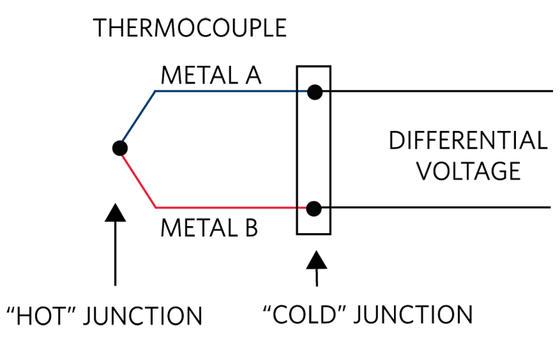
\includegraphics[width=0.8\textwidth]{Thermocouple.jpg}
            \caption{Thermocouple setup}
      \end{figure}

      \end{minipage}\\

      \hline      
      \begin{minipage}[b]{0.6\textwidth}
        \begin{figure}[H]
              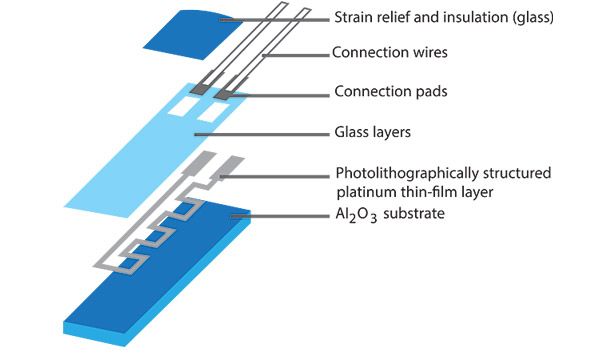
\includegraphics[width=1\textwidth]{RTD.jpg}
              \vspace{-5mm}
              \caption{RTD}
              \vspace{2mm}
        \end{figure}
      \end{minipage}
         &  
        \begin{minipage}[b]{0.39\textwidth}
            \textbf{Resistance Temperature Detectors (RTDs)}, measure temperature changes by correlating the resistance of the device element and temperature. An RTD consists of a film for greater accuracy, a wire wrapped ceramic or a glass core \cite{Temprature_sensor}. 
            \vspace{13mm}
        \end{minipage}\\
        \hline
    \end{tabular}
    \caption{Types of temperature sensors}
\end{table}

\newpage
\section{Communication}
Traditionally when connecting multiple servomotors to a microcontroller, each servo must be individually connected to the micro, and each servo must individually be connected to the power supply. This can result in long masses of wires when multiple servomotors are used in one project, seen in Figure 2.16. This also limits the number of servomotors that can be controlled at a time to the number of GPIO pins available on the microcontroller.

\begin{figure}[H]
\centering
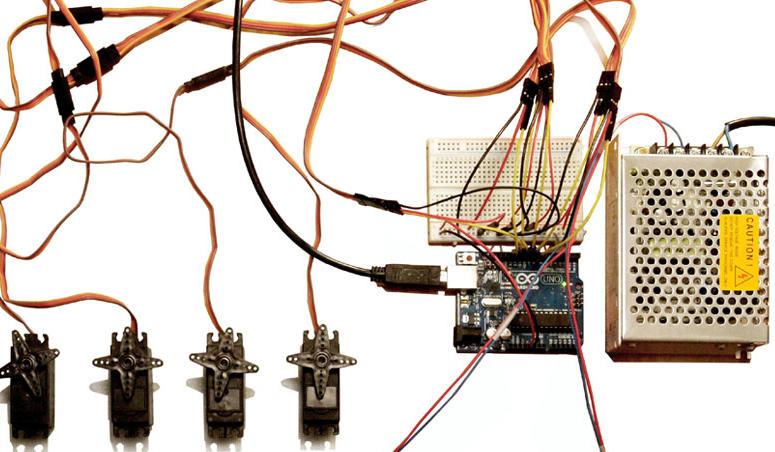
\includegraphics[width=0.4\textwidth]{toomanywires.jpg}
\caption{Multiple servomotors connected to one microcontroller\cite{toomanywires}}
\label{fig:typset}
\end{figure}

The controller board that will be designed to enable that the servo motors to be connected in series and be able to communicate using the RS485 differential serial communication standard. This will allow for communication over a longer distances with a high noise rejection for increased accuracy. This enables the master to effectively communicate to each individual slave a certain position value and request information such as current drawn or temperature at the motor from it in return. The Master and Slave servo inter-connection can be seen below in Figure \ref{fig:servoconnection} \newline

\begin{figure}[H]
\centering
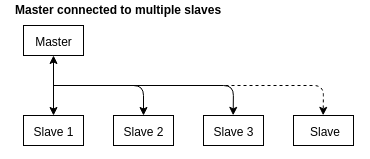
\includegraphics[width=0.6\textwidth]{master_slave.png}
\caption{Servo inter-connection}
\label{fig:servoconnection}
\end{figure}

The RS485 standard is a hardware protocol that will require that the microcontroller interacts with a transceiver which will be able to facilitate the communication. 


\newpage
\subsection{Serial communication}
Serial communication is the process of sending data one bit at a time, from one device to another sequentially over a communication channel or a computer bus \cite{serial_comms}. Communication is accomplished using 3 lines. (1) Ground (2) Transmit and (3)Receive. 

Serial communication can be synchronous or asynchronous. What this means is that the communicating devices either run off their own clocks and before hand decide on a common speed at which to communicate, this is asynchronous communication.  Or they will run off a common clock which will in turn give them a common communication speed,  this is synchronous communication. Asynchronous communication allows for information to be transmitted and received simultaneously. This is know as Full Duplex communication. Where as synchronous communication is Half Duplex communication and only one device can transmit information at a time. Serial communication can be used over much greater distances in comparison to other forms of communication, such as parallel communication, making it ideal in applications when communicating between devices that are far apart . 

\textbf{Serial communication is made of four parts :}
\begin{enumerate}
\item{\textbf{Baud rate}}
is the speed at which the communication occurs and it indicates the bits the number of bits transferred per second. Baud rate can also be read as the frequency of the clock needed for sampling, for example 3000 baud would mean the clock is running at 3kHz.
\item{\textbf{Data bits}}
are bits of information that needs to be transmitted.
\item{\textbf{Stop bits}}
are used to indicate the end of the communication for a single packet.
\item{\textbf{Parity}}
is used for error checking when using serial communication. There are four types of parity. Even, odd, marked, and spaced. When using even or odd parity the last bit after the data will be set to 0 or 1. Depending if it is even or odd parity. Then when a message is received its parity can be checked to check its accuracy. This can be used to detect noise and whether the communicating devices clocks are out of sync.

\end{enumerate}
\begin{figure}[H]
\centering
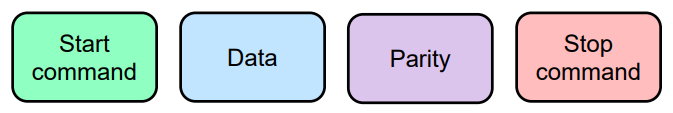
\includegraphics[width=0.6\textwidth]{serial.png}
\caption{Basic structure of a serial message}
\end{figure}

\newpage
\subsection{Recommended Standards}
When communicating using serial communication a Recommended Standard (RS) is typically used for easy connection between different devices. These standards use the Universal Asynchronous Receiver Transmitter (UART) hardware interface to facilitate the communication. Usually a UART is part of an integrated circuit (IC) and the signal level shifting needs to be handled by a driver circuit external of the UART. When communicating using a RS, a hardware interface is required in order to do the voltage level shifting. These components are known as level shifting transceivers. 

A simplified diagram of the implementation of asynchronous serial communication between two devices can be seen below in Figure 2.19.
\begin{figure}[H]
\centering
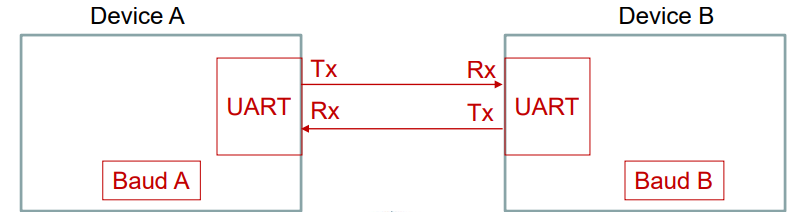
\includegraphics[width=0.8\textwidth]{UART.png}
\caption{UART communication between two devices }
\label{fig:comms}
\end{figure}

\textbf{Common Standards :}
\begin{enumerate}
\item{\textbf{RS232}}
Designed to work over a distance of up to 15 meters. The maximum baud rate is 19.2k. A logic level of -3v and less represents a 1 and 3v and more represents 0 \cite{RS232}.

\item{\textbf{RS422}}
Introduced to enable higher data rates than what was possible with RS-232 using differential transmitters and receivers. Works over a distance of up to 15m \cite{RS422}. 

\item{\textbf{RS485}}
RS-485 uses differential serial communication. Differential communication transmits information using two complementary signals over a twisted pair of conductors. Any external electromagnetic interference will then effect both conductors in the same way. Since the receiving circuit detects only the difference between the pair of conductors, the signal can be communicated more clearly and over greater distances \cite{Differential communication}. allowing for there to be up to 32 devices connected to a single serial communication line \cite{RS485}. 
\end{enumerate}

\newpage
\section{Buck Converter}
\vspace{-5mm}
According to Joule’s first law. The electrical current passing through a conductor  will generate heat with power that is proportional to resistance of the conducter and square of the current, $P=I^2\times R$. Therefore, in order to minimise power loss, the current drawn is reduced. In order to still transmit the same amount of power with the lower current, the voltage is increased as $P=V\times I$ \cite{High_voltage}. 

That is, in order keep power the same, while transmitting lower current, the voltage must be increased. Thus in order to be able to efficiently supply power to multiple servomotor controller boards, all the boards will be connected to a supply voltage in the range of 5V to 40V. Each board will have its own on-board buck converter to step down the voltage and step up the current in order to drive the servomotor and other components.

The power supply required for the designed board must be able to power the servo motor as well as the other on board components. This means that the supply must be able to handle the total current requirement of the board while still supplying the 5V required by the servo motor. Any other voltage requirements in the circuit will require a voltage regulator for further regulation.  

When considering the buck converter, the power demands of the servomotor was the greatest. The current drawn by the rest of the components was almost negligible in comparison. Table 2.5 was used to create an idea of a typical servomotors power consumption characteristics. This was used to help determine the current requirements of the designed buck converter.
\vspace{2mm}
\begin{table}[H]
        \centering
        \begin{tabular}{|c|c|c|c|}
        \hline
         \textbf{\underline{Name}}  & \textbf{\underline{Weight(g)}}   & \textbf{\underline{Stall Torque($\frac{kg}{cm}$)}} & \textbf{\underline{Stall Current(A})}\\
          MG90S   & 13.4 & 1.8  & 0.2  \\
          MG90    & 14   & 2    & 0.48 \\
          SG-5010 & 39   & 5.5  & 0.6  \\
          MG996R  & 55   & 9.4  & 2.5  \\
          MG946R  & 55   & 10.5 & 1.2  \\
          MG958   & 65   & 18   & 1.6  \\
          \hline
        \end{tabular}
        \caption{Current requirements of various servomotors}
\end{table}
\vspace{-5mm}
It was determined that the buck converter needed to be able supply 5V while outputting up to 4A worth of current in order to be able to run a range of different servo motors at stall torque as well as sufficiently power the rest of the circuit.

\subsection{Design Procedure}
Buck converters are a type of switch mode power supply that step down a higher voltage to a lower voltage. This is achieved through high frequency switching of the circuit with the source voltage with the help of a few added necessary components. 

The kind of switching required by the buck converter is typically achieved with a high speed MOSFET. A microcontroller supplies a PWM signal of the right frequency to the gate of the MOSFET, the duty cycle of the PWM signal determining the length of time of which the switch will stay open and closed. A basic buck converter circuit can be seen in Figure \ref{typbuck}.
\begin{figure}[H]
    \centering
    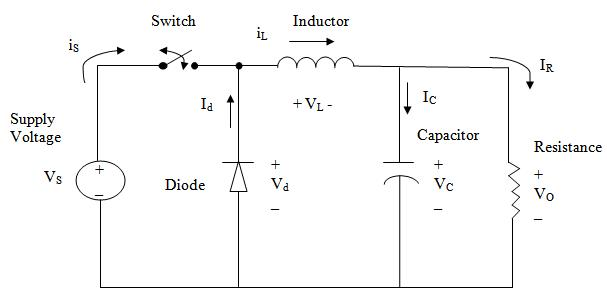
\includegraphics[width=0.85\textwidth]{buckconverter.JPG}
    \caption{A basic buck converter circuit \cite{buckconverter}}
    \label{typbuck}
\end{figure}
\vspace{-2mm}
In order to sufficiently meet design requirements, the design procedure requires that the following parameters need to be known or calculated :
\vspace{2mm}
\begin{table}[H]
        \centering
        \begin{tabular}{l l}
         \textbf{Parameters chosen}  & \textbf{Parameters needing to be calculated}\\
         $V_{IN(max)}$ = maximum input voltage & D =duty cycle\\
         $V_{OUT}$ = desired output voltage & \triangle _L = Inductor Ripple Current\\
         $I_{LIM(min)}$ = minimum current to the switch & $I_{MAXOUT} $ = Maximum IC output current \\
         $f_s$ = minimum switching frequency of IC &L = calculated inductor value \\
         $\mu = $ efficiency of the converter&$I_{SW(max)}$ = Maximum switch current\\
        \end{tabular}
        \vspace{2mm}
        \caption{Buck converter parameters}
\end{table}
\newpage
\subsection{Calculations}
\vspace{-2mm}
Once the desired buck converter IC, and input output parameters have been chosen. The following calculations can be done in order to solve for the components required to build the buck converter circuit. The calculations used for the design process of the buck are based on those found in the application  report  "Basic Calculation of a Buck Converter's Power Stage", made by Texas Instruments \cite{buck_calculations}.

\subsubsection{Maximum Switch Current}
\vspace{-6mm}
The first step to calculating the switch current is to determine the duty cycle, D, for the maximum input voltage:
\vspace{-5mm}
\begin{figure}[H]
    \centering
    $\mathbf{D = \frac{V_{OUT}}{V_{IN(max)}\times \mu}}$
\end{figure}
\vspace{-5mm}
The inductor ripple current is determined by chosen an inductor specified in the buck converters data sheet:
\vspace{-5mm}
\begin{figure}[H]
    \centering
    $\mathbf{\triangle I_L = \frac{(V_{IN(max)-V_{OUT}\times D})}{f_s\times L}}$ 
\end{figure}
\vspace{-5mm}
It needs to be determined if the chosen buck converter IC can deliver the required maximum output current:
\vspace{-5mm}
\begin{figure}[H]
    \centering
    $\mathbf{I_{MAXOUT} = I_{LIM(min)} - \frac{\triangle  I_L}{2}}$
\end{figure}
\vspace{-6mm}
If the maximum output current is above the maximum output current required for the device, the maximum switch current of the system must be calculated in order to determine the peak current that the inductor, switch and external diode must be able to withstand: 
\vspace{-5mm}
\begin{figure}[H]
    \centering
    $\mathbf{I_{SW(max)} = \frac{\triangle I_L}{2} + I_{OUT(MAX)}}$ 
\end{figure}
\vspace{-5mm}

\subsubsection{Inductor Selection}
\vspace{-6mm}
The buck converters data sheet will have a range of recommended inductor values, the higher the maximum output inductor, the higher the maximum output current due to reduced ripple. If no recommended inductor is given in the buck converters data sheet the following equation can be used:
\begin{figure}[H]
    \centering
    $\mathbf{L = \frac{V_{OUT} \times(V_{IN} - V_{OUT})}{ \triangle I_L \times{f_s} \times{ V_{in}}}}$
\end{figure}


\newpage
\subsubsection{Rectifier Diode}
\vspace{-2mm}
The chosen rectifier diode needs to be able to handle the fast switching and the current loads experienced during operation. The foreword current rating of the rectifier can be calculated using:
\vspace{-2mm}
\begin{figure}[H]
    \centering
    $\mathbf{I_F = I_{OUT(MAX)}\times(1-D)}$ 
\end{figure}
\vspace{-6mm}
Schottky diodes can be used to reduce the losses experienced, due to there fast switching capabilities and the low voltage drop across the diode.
The power that the chosen diode needs to be able to safely dissipate is calculated:
\begin{figure}[H]
    \centering
    $\mathbf{P_D = I_F\times V_F}$ 
\end{figure}
\vspace{-5mm}
\subsubsection{Output Voltage}
\vspace{-2mm}
Most buck converters set the output voltage with a resistive feedback divider network with resistors $R_1$ and $R_2$. This determines the feedback voltage $V_{FB}$. With $V_{OUT}$ the desired output voltage and the feedback bias current, $I_{FB}$, the resistors for the voltage divider can be calculated:
\begin{figure}[H]
  \begin{minipage}[b]{0.48\textwidth}
      \begin{figure}[H]
    \centering
    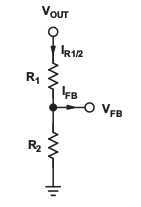
\includegraphics[width=0.35\textwidth]{Voltage_set.jpg}
    \caption{Resistive Divider}
    \end{figure}
  \end{minipage}
  \hfill
  \begin{minipage}[b]{0.48\textwidth}
    \begin{figure}[H]
    \hspace{10mm}
    $\mathbf{R = \frac{V_{FB}}{I_{R\frac{1}{2}}}}$ 
    \end{figure}
    \begin{figure}[H]
    \hspace{10mm}
    $\mathbf{R_1 = R_2 \times{( \frac{V_{OUT}}{V_{FB}} - 1)}}$ 
    \end{figure}
    \vspace{16mm}
  \end{minipage}
\end{figure}

\subsubsection{Input Capacitor}
\vspace{-2mm}
The minimum value of the input capacitor is normally given in buck converter ICs the data sheet. This is the minimum value necessary to stabilise the input voltage due to the peak current requirement of a switching power supply.

\newpage
\subsubsection{Output capacitor}
\vspace{-5mm}
The recommended value for the output capacitor is usually given in the buck converter ICs data sheet. The output capacitors value for a desired output voltage ripple is given by:
\vspace{-5mm}
\begin{figure}[H]
    \centering
    \large
    $\mathbf{C_{OUT(min)} = \frac{\triangle I_L}{\times f_s \times \triangle I_L}}$
\end{figure}
\vspace{-7mm}
If the output capacitors selection is based in transient response and not steady state ripple, the following formula can be used to calculate the output capacitance required for a desired minimum overshoot: 
\begin{figure}[H]
    \centering
    \large
    $\mathbf{C_{OUT(min),OS} = \frac{\triangle I_{OUT} \times L}{2 \times f_s V_{OUT} \times V_{OS}}}$
\end{figure}

\vspace{-9mm}
\section{Voltage Regulator IC}
\vspace{-5mm}
The on board components will run at the same or lower voltage than that of the servomotor and in order to step down the voltage an on board voltage regulator IC will be required.

Linear voltage regulators make use of a BJT or MOSFET device controlled by a high gain differential amplifier. The output voltage is compared to a reference voltage created by resistors R1 and R2 in Figure \ref{RESDIV} The output voltage is constantly adjusted to match this reference voltage in order to maintain a regulated output.  

Although the implementation of a linear regulator is simple, it is often a more inefficient method of regulation. The transistor or MOSFET acts as a resistor and any excess electrical energy is dissipated as heat\cite{linear_regulator}
\vspace{-4mm}.
\begin{figure}[H]
    \centering
    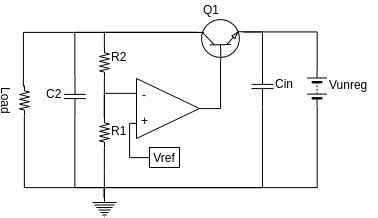
\includegraphics[width=0.55\textwidth]{Linear_Voltage_Regulator.jpg}
    \caption{Typical voltage regulator IC}
    \label{RESDIV}
\end{figure}
\vspace{-8mm}
It is common to find fixed three terminal linear regulators that generate a fixed standard voltage needed by common microcontrollers and peripherals such as the 3.3V or 5V without requiring any external components.

\newpage
\section{Related projects}
\subsection{Dynamixel}
The Dynamixel is an energy efficient high performance actuator that includes a controller, motor driver and network capabilities allowing multiple motors to be communicated to on a single channel.
\begin{figure}[H]
\centering
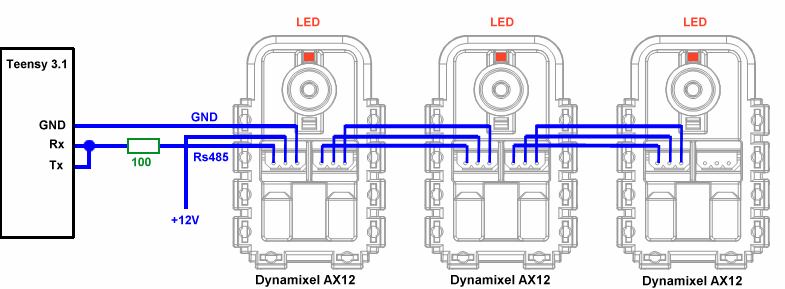
\includegraphics[width=0.7\textwidth]{Dynamixel.png}
\caption{Dynamixel connectors \cite{Dynamixel}}
\end{figure}

The Dynamixel allows for position and velocity control, as well as current based torque control of a brushless DC motor.  This allows for 360\degree  rotation with six standard operating modes ,although it can be programmed specifically for each application, this allowing for wide range implementation. Temperature and current tracking allow for shutdown protection. Due to high cost only larger companies and well funded organisations tend to have access to these devices. A standard Dynamixel actuator can cost up to R4500.\newline
 
\begin{figure}[H]
\centering
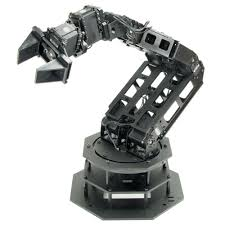
\includegraphics[width=0.35\textwidth]{Dynamixel_app.jpg}
\caption{Dynamixel based robotic arm  \cite{Dynamixel}}
\end{figure}


\newpage
\subsection{Odrive}
Odrive is a high performance servomotor controller board which uses a high resolution encoder with brushless DC motors in order to achieve  high accuracy position and velocity control. \newline

\begin{figure}[H]
\centering
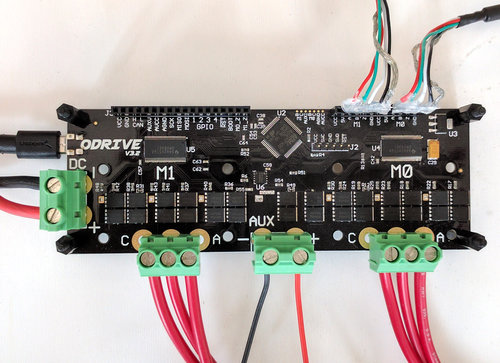
\includegraphics[width=0.5\textwidth]{odrive_board.jpg}
\caption{Odrive controller board\cite{Odrive}}
\end{figure}

The servomotor controller board can drive to motors. It allows for current, position and velocity control. Motor breaking can be achieved with a brake resistor and the board supports regenerative breaking. Communication with the board can be achieved with multiple interfaces, such as USB, UART, PWM and CAN. Although the Odrive is cheaper than the Dynamixel, it still costs R1800 for just the controller board.

\begin{figure}[H]
\centering
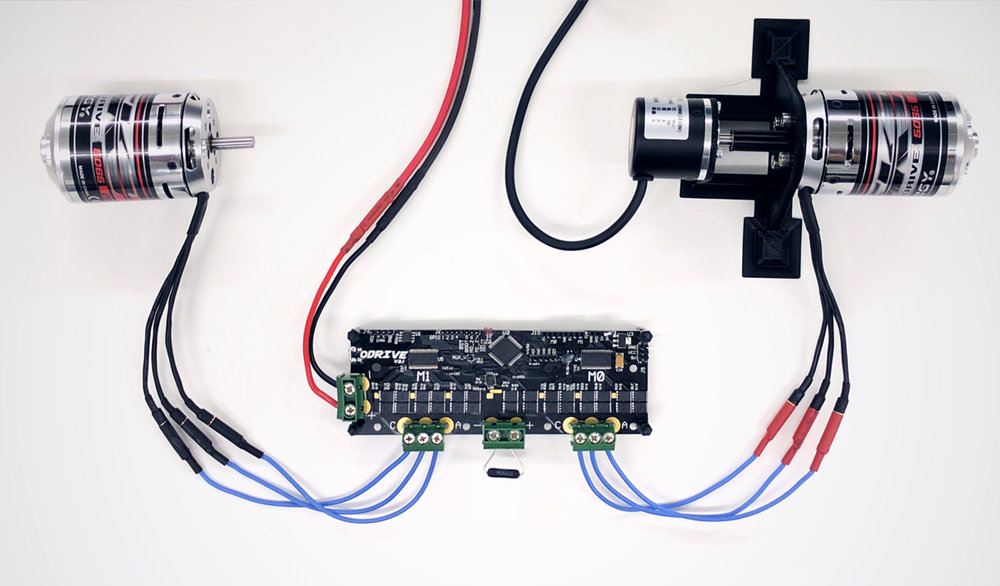
\includegraphics[width=0.6\textwidth]{Odrive.jpg}
\caption{Odrive setup\cite{Odrive}}
\end{figure}

